\documentclass[11pt, oneside]{article}   	% use "amsart" instead of "article" for AMSLaTeX format
\usepackage{geometry}                		% See geometry.pdf to learn the layout options. There are lots.
\geometry{letterpaper}                   		% ... or a4paper or a5paper or ... 
%\geometry{landscape}                		% Activate for for rotated page geometry
%\usepackage[parfill]{parskip}    		% Activate to begin paragraphs with an empty line rather than an indent
\usepackage{graphicx}				% Use pdf, png, jpg, or eps§ with pdflatex; use eps in DVI mode
								% TeX will automatically convert eps --> pdf in pdflatex		
\usepackage{amssymb}

\title{Mining Revisions to Questions and Answers on StackExchange.com}
\author{Felix Grezes and Michelle Morales}
\date{\today}							% Activate to display a given date or no date

\begin{document}
\maketitle

\section{Introduction}
The main premise of this project was to work with data from the Stack Exchange website (stackexchange.com). This site is an aggregation of question and answer sites on diverse topics consisting of 110 question and answer sites, 4.5 million users, 7.9 million questions, and 14.1 million answers. Each question on stack exchange is given a webpage, where users can provide answers. The site provides a dynamic and interactive environment for users: questions are voted on and scored by users, answers are ranked on usefulness, and revisions and comments can be made on both questions and answers. Much like Wikipedia, Stack Exchange dates and archives every revision and makes this data accessible. Our goal was to collect and analyze this revision data suggesting how it may be used to aid in Natural Language Processing(NLP) tasks, specifically addressing edit classification and how classification may then be used to generate edit suggestions. OUTLINE PAPER...

\section{Related Work}
Wikipedia's revision history data has been used many times to aid a number of NLP tasks. Wikipedia is attractive because of its dynamic nature and size; it's constantly edited, and is now a collection of millions of articles. Thus, it provides rich data for researchers, and has been implemented successfully to help improve tasks in sentence compression (Yamangil and Nelken, 2008), edit classification (Max and Wisniewski 2010),  and machine translation (Wubben et. al, 2012). Stack Exchange mirrors Wikipedia in many ways and therefore can also be useful data to collect. In addition, Stack Exchange includes long and detailed questions, something that Wikipedia, in fact, lacks. The goal of our work closely resembles work done by Bonner and Monz, who introduce an approach for automatically distinguishing between factual and fluency edits in document revision histories from Wikipedia (Bonner and Mons 2013). Their approach is based on supervised machine learning using language model probabilities, string similarity of user edits, comparison of part-of-speech tags and named entities, and a feature set extracted from unlabeled user edits. Our work, also focuses on distinguishing between factual and fluency edits, but differs in our use of Stack Exchange data, the heuristics we use for classification and our suggestion of an unsupervised learning approach. 

\section{Data}
\subsection{Collection}
To collect our data we wrote a web crawler to accumulate, from the 110 question and answer sites of Stack Exchange, a total of 6500 question and answer pairs. The data for each question and answer pair consists of text (title, question text, answer text), tags(topic of question/answer), score, rank, revision edits, and metadata (images, code, links). These attributes of the data we then choose to use as features in our first task: correlating a question/answer's score with its features. 

\subsection{Preliminary analysis}
Before we could address edit classification and subsequently edit suggestion we explored what factors may be influencing our data. First, we considered what effect time may have: as the age of question increases what happens to the score? Figure 1 shows our findings, demonstrating that time could be the main factor in making a good question. Next, we plotted score against its count. Figure 2, shows us that good questions are rare. Our preliminary results suggest that due to scarcity and time effect it will be unlikely to find a correlation between a question's score and its features. \\

\centering 
Figure 1
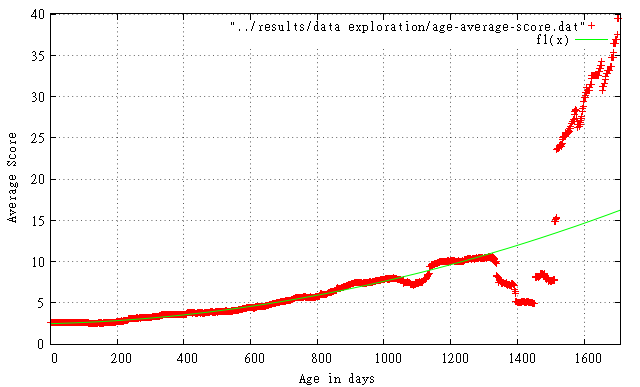
\includegraphics[height=2.8in, width=\textwidth]{age-average-score}

Figure 2
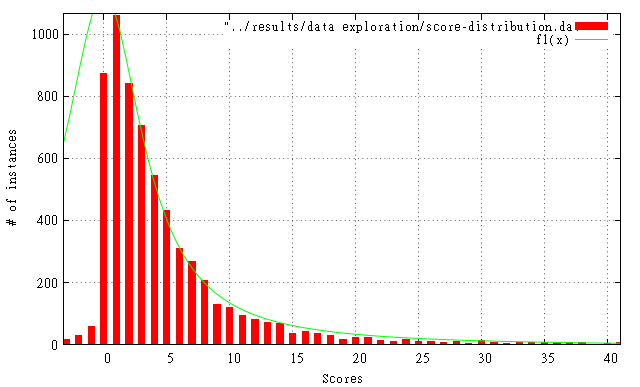
\includegraphics[height=3in, width=\textwidth]{score-instances.png}

\raggedright

\section{Task 1}
\subsection{Correlate Score with Features}
The goal of our first task was to find out if the textual information (text, title, tags) were responsible for high scores. As our preliminary data suggested, this was probably unlikely.  We tested different representations: bag-of-words, N-grams, stemming, and no stemming. These representations were used on the text of the question/answer pair; the text of the data consisted of the title of the question, the question itself, the tags of the question, and the text from every answer. It is not until Task 2 that we include the revision text, because in this task we are only concerned with the score, which can only fairly be associated with the most current version of the text, not its revisions. 
\subsection{Results}
We then ran a Sequential Minimal Optimization (SMO) algorithm on Weka for each representation of the data and found a low correlation on all test sets: about 1\%. As predicted, the text is not predictive of the score, implying that perhaps either the age or the semantics of the question is what is indicative of its usefulness. 

\section{Task 2}
\subsection{Classifying Edits} 
Following the terminology used by Bronner and Monz, we wish to classify our edits into two main groups:{ \itshape fluency edits}, which improve the style or readability of the text, and {\itshape factual edits}, which alter the meaning of the text (Bronner and Monz 2013).   From the 6500 question and answer pairs collected during data collection we extract about 20,000 edit pairs.  Table 1 below shows examples of the edit pairs collected. \\

\centering
Table 1
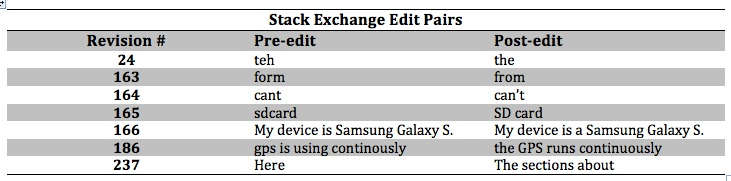
\includegraphics[width=\textwidth]{table1-editpairs}

\raggedright
Our edit pairs vary in length from 1 character, to one word, to a few words, to a full sentence. Sometimes a correction is a complete deletion, an addition, or a substitution. In Table 1, revision 24 and revisions 163-167 are examples of fluency edits. Where revision 186 and 237 are factual edits. It is fair to assume that, fluency edits consist of small changes, such as spelling corrections, capitalizations, and punctuation. Factual edits, then consist of longer edits.This basic intuition, follows from Bronner and Monz, "longer edits are likely to be factual and shorter edits are likely to be fluency edits" (Bonner and Monz 2013). The baseline method we therefore use is character-level edit distance (Levenshtein, 1966) between pre- and post-edited text. The simplest edit to categorize and identify are spelling errors, using a spell checker we were able to easily find and compile a list of spelling corrections.

Once we set aside all the edits that could be simply categorized as spelling, we started inspecting the more interesting edits. To this end we searched for the most common deletion-addition pairs that also had an edit distance greater than 1. 

\subsection{Results and Possible Suggestions for Revisions}
Of the 20000 edit pairs we extracted from our data, approximately 3000 were found to be spelling correction by our simple spell-checker. Of the remaining 17000, about 600 appeared more than once and had an edit distance greater than 1. From a manual inspection of these 600 pairs, the following categories emerged.
\newline

{\bfseries Spelling Errors:} some of the edit pairs captured are simply spelling errors that were missed by the previous classification. These can be grammatical: your $\rightarrow$ you're; semantical: right $\rightarrow$ write. Suggesting these kind of edits seems difficult, as they really depend the meaning of the sentence.\\

{\bfseries Stylistic Improvements:} some of the pairs, such as: im $\rightarrow$ I'm, pants $\rightarrow$ trousers, virtually every $\rightarrow$ many; are examples of stylistic improvement that almost certainly improve the question. This type of revision should be suggested and is a path to explore in the future.\\

{\bfseries Named Entities:} interestingly, a number of revisions found are related to named entities. Identifying these give us a database entities and their correct spelling. Suggesting this proper spelling should be an improvement to the question in most cases. This result could incidentally be useful in a related NLP task of Named Entity Recognition.\\
Some examples of edits related to named entities are: cayogenMod $\rightarrow$ CyanogenMod, MAC OSX $\rightarrow$ Mac OS X,torrent $\rightarrow$ BitTorrent, stackexchange $\rightarrow$ Stack Exchange, rainbow dash $\rightarrow$ Rainbow Dash and a number more. We feel this to be a promising area of future studies.

{\bfseries Miscelaneous:} a fair number of re-occurring edit pairs are not interesting, though it is surprising that they have occurred at least twice, seeing how esoteric some are. Some are correction of large mistakes, and the addition is not related to the deletion. Some are symbol manipulation, making them difficult to interpret out of context: \$n\$ $\rightarrow$ \$n=3\$.\\
Some though seems to be potentially interesting: to speech $\rightarrow$ -to-speech, although this particular one could be considered a stylistic improvement.


\section{Conclusion}
\section{Future Work}



\end{document}  